\documentclass[aps,twocolumn,prl,showpacs,preprintnumbers,amssymb,english]{revtex4-2}
\usepackage{amsmath, amssymb}
\usepackage{color}
\usepackage[T1]{fontenc}
\usepackage{tikz}
\usepackage{tikz-feynman}

\begin{document}

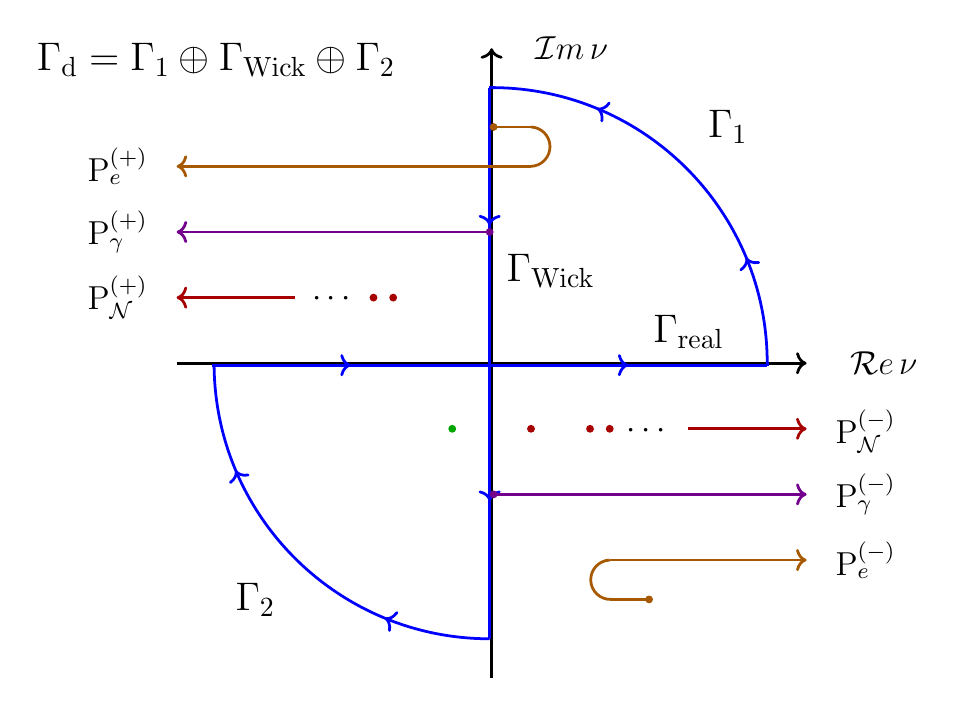
\begin{tikzpicture}
% defining arrow decorations
[
	decoration={%
	markings,
	mark=at position 0.25 with {\arrow[line width=1pt]{>}},
	mark=at position 0.75 with {\arrow[line width=1pt]{>}},
	}
]
% defining variables
\def\deltaaxis{0.025}
\def\contourradius{3.5}
\def\deltapolesnuclear{0.833}
\def\deltapolesphoton{1.666}
\def\deltapoleselectron{2.5}
% drawing axes
\draw [ ->, line width=1.0 ] (-4,0) -- (4,0) node[ right, font=\large ] {$ \quad \mathcal{R}e \, \nu $};
\draw [ ->, line width=1.0 ] (0,-4) -- (0,4) node[ right, font=\large ] {$ \quad \mathcal{I}m \, \nu $};
\node [ font=\Large ] at ( -\contourradius, \contourradius*1.1 ) {$ \Gamma_{ \mathrm{d} } = \Gamma_{ 1 } \oplus \Gamma_{ \mathrm{Wick} } \oplus \Gamma_{ 2 } $};
%%%%
% drawing the deformed contour
%%%%
% arc in first quadrant
\path [ draw, blue, line width=1.0, postaction=decorate ] ( \contourradius, 0 ) arc ( 0 : 90 : \contourradius );
\path [ draw, blue, line width=1.0 ] ( 0, \contourradius ) -- ( -\deltaaxis - 0.01, \contourradius );
\node [ font=\Large ] at ( \contourradius - 0.5, \contourradius - 0.5 ) {$ \Gamma_{ 1 } $};
% arc in third quadrant
\path [ draw, blue, line width=1.0, postaction=decorate ] ( -\deltaaxis, -\contourradius ) arc ( 90 : 0.5 : -\contourradius );
\node [ font=\Large ] at ( -\contourradius + 0.5, -\contourradius + 0.5 ) {$ \Gamma_{ 2 } $};
% path along real axis
\path [ draw, blue, line width=1.0, postaction=decorate ] ( -\contourradius - 0.05, -\deltaaxis ) -- ( \contourradius, -\deltaaxis );
\path [ draw, blue, line width=1.0 ] ( \contourradius, -\deltaaxis - 0.01) -- ( \contourradius, 0.0 );
\node [ font=\Large ] at ( \contourradius - 1.0, 0.4 ) {$ \Gamma_{ \mathrm{real} } $};
% path along imaginary axis
\path [ draw, blue, line width=1.0, postaction=decorate ]  ( -\deltaaxis, \contourradius ) -- ( -\deltaaxis, -\contourradius );
\node [ font=\Large ] at ( 0.75, \contourradius/3 ) {$ \Gamma_{ \mathrm{Wick} } $};
%%%%
% nuclear propagator poles
%%%%
\draw[ fill=green!65!black ] ( -0.5, -\deltapolesnuclear ) coordinate [ circle, fill, inner sep=1pt ] (np0);
% negative real axis nuclear poles ( W x EM )
\draw[ fill=red!65!black ]
( -1.25, \deltapolesnuclear ) coordinate [ circle, fill, inner sep=1pt ] (np2)
( -1.5, \deltapolesnuclear ) coordinate [ circle, fill, inner sep=1pt ] (np3);
\node [ font=\large ] at ( -2.0, \deltapolesnuclear - \deltaaxis ) {$\cdots$};
\draw[ ->, line width=1.0, red!65!black ] ( -2.5, \deltapolesnuclear ) -- ( -4, \deltapolesnuclear );
\node [ font=\large ] at ( -4.75, \deltapolesnuclear ) {$ \mathrm{P}^{(+)}_{ \mathcal{N} } $};
\draw[ fill=red!65!black ]
( 0.5, -\deltapolesnuclear ) coordinate [ circle, fill, inner sep=1pt ] (np2)
( 1.25, -\deltapolesnuclear ) coordinate [ circle, fill, inner sep=1pt ] (np3)
( 1.5, -\deltapolesnuclear ) coordinate [ circle, fill, inner sep=1pt ] (np4);
\node [ font=\large ] at ( 2.0, -\deltapolesnuclear - \deltaaxis ) {$\cdots$};
\draw[ ->, line width=1.0, red!65!black ] ( 2.5, -\deltapolesnuclear ) -- ( 4, -\deltapolesnuclear );
\node [ font=\large ] at ( 4.75, -\deltapolesnuclear - \deltaaxis ) {$ \mathrm{P}^{(-)}_{ \mathcal{N} } $};
%%%%
% photon propagator poles
%%%%
\draw [ fill=red!45!blue ] ( \deltaaxis, -\deltapolesphoton ) coordinate [ circle, fill, inner sep=1pt ] (pp2);
\draw [ ->, line width=1.0, red!45!blue ] ( 0, \deltapolesphoton ) -- ( -4, \deltapolesphoton );
\node [ font=\large ] at ( -4.75, \deltapolesphoton ) {$ \mathrm{P}^{(+)}_{ \gamma } $};
\draw [ fill=red!45!blue ] ( -\deltaaxis, \deltapolesphoton ) coordinate [ circle, fill, inner sep=1pt ] (pp1);
\draw [ ->, line width=1.0, red!45!blue ] ( 0, -\deltapolesphoton ) -- ( 4, -\deltapolesphoton );
\node [ font=\large ] at ( 4.75, -\deltapolesphoton ) {$ \mathrm{P}^{(-)}_{ \gamma } $};
%%%%
% electron propagator poles
%%%%
\draw [ fill=red!65!green ] ( \deltaaxis, \deltapoleselectron + 0.50 ) coordinate [ circle, fill, inner sep=1pt ] (pp1);
\draw [ red!65!green, line width=1.0 ] ( 0.5, \deltapoleselectron ) arc ( 92 : 268 : -0.25);
\draw [ red!65!green, line width=1.0 ] ( 0.0, \deltapoleselectron + 0.50 ) -- ( 0.5, \deltapoleselectron  + 0.50 );
\draw [ ->,  red!65!green, line width=1.0 ] ( 0.5, \deltapoleselectron ) -- ( -4.0, \deltapoleselectron );
\node [ font=\large ] at ( -4.75, \deltapoleselectron ) {$ \mathrm{P}^{(+)}_{ e } $};
\draw [ fill=red!65!green ] ( 2.0, -\deltapoleselectron - 0.50 ) coordinate [ circle, fill, inner sep=1pt ] (pp2);
\draw [ red!65!green, line width=1.0 ] ( 1.5, -\deltapoleselectron ) arc ( 92 : 272 : 0.25);
\draw [ red!65!green, line width=1.0 ] ( 2.0, -\deltapoleselectron - 0.50 ) -- ( 1.5, -\deltapoleselectron  - 0.50 );
\draw [ ->,  red!65!green, line width=1.0 ] ( 1.5, -\deltapoleselectron ) -- ( 4.0, -\deltapoleselectron );
\node [ font=\large ] at ( 4.75, -\deltapoleselectron ) {$ \mathrm{P}^{(-)}_{ e } $};
\end{tikzpicture}

\end{document}